%! Author = leona
%! Date = 09/02/24
% !TeX root = ../thesis-main.tex

\chapter{Design}
\label{chap:design}
This chapter aims to give the reader a comprehensive view of this thesis' design. First, we will present the architectural design of the system, then we will shift the focus on
the detailed design, where the system will also be described in terms of behavior and interaction.

\section{Architectural Design}
\label{sec:architectural-design}
In this section, we will present and discuss RuFi's architectural design, shown in figure \ref{fig:rufi-architecture}.

\begin{figure}[ht]
    \centering
    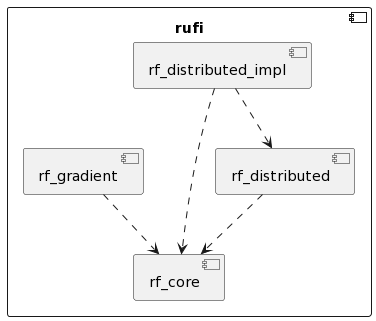
\includegraphics[width=0.8\textwidth]{figures/diagrams/img/rufi-architecture.png}
    \caption{RuFi's architectural design}
    \label{fig:rufi-architecture}
\end{figure}

In the figure, we can see the following components:

\begin{itemize}
    \item \textbf{rf-core}: this component defines key abstractions, such as the fundamental aggregate operators, builtins and a virtual machine;
    \item \textbf{rf-distributed}: this component defines concepts related to the distributed execution of aggregate programs.
          In particular, it defines core abstractions related to networking and message passing, as well as an implementation of the computational model discussed in \ref{par:comp-model};
    \item \textbf{rf-distributed-impl}: this component exposes a standard implementation for the concepts defined in \textbf{rf-distributed}.
          The choice of separating the abstraction definitions and the implementations will be discussed in section \ref{subsec:rufi-distributed};
    \item \textbf{rf-gradient}: this component is a library exposing the gradient algorithm as an aggregate program.
    \item \textbf{rufi}: this component, which serves as the main user interface with the framework, re-exports all the other components under a coherent namespace.
\end{itemize}

\subsection{RuFi Core}

\subsection{RuFi Distributed}
\label{subsec:rufi-distributed}

\section{Detailed Design}
\label{sec:detailed-design}

\subsection{Behavior}

\subsection{Interaction}